% !TeX document-id = {fb298762-8474-4a7b-90a0-a0c749091c0f}
%!BIB program = biber
\documentclass[12pt,twoside]{../../mitthesis}
% \documentclass[12pt,a4paper]{article}
% \documentclass{minimal}
%%%%%%%%%%%%%%%%%%%%%%%%%%%%%%%%%%%%%%%%%%%%%%%%%%%%%%%%%%%%%%%%%%%%%%%%%%%%%%%%%%%%%%%%%%%%
%%%%%%%%%%%%%%%%%%%%%%%%%%%%%%%%%%%%%%%%%%%%%%%%%%%%%%% IMPORTS
\usepackage{hyperref}
\usepackage{amsmath,amssymb,amsfonts}
\usepackage{mathtools}						% Load after amsmath and mathspec. Needed for custom delimiters
\usepackage{algorithmic}
\usepackage{graphicx}
\usepackage{textcomp}
\usepackage{subcaption}
\usepackage[shortlabels]{enumitem}
\usepackage[ruled,vlined]{algorithm2e}
\usepackage{float}
\usepackage{wrapfig}
% \usepacakge{color}						
\usepackage{xcolor}
\usepackage{setspace}
\usepackage{wasysym}
\usepackage{xspace}							% Provides \xspace 

\usepackage{lipsum}  						% Remove this, it's for the template only
\usepackage{tabularx}  						% Used in the template. Nice package, but use with care. Remove by default 
\usepackage{etoolbox}						% Provides \iftoggle
% \usepackage[mathletters]{ucs}
\usepackage[utf8]{inputenc}
%%%%%%%%%%%%%%%%%%%%%%%%%%%%%%%%%%%%%%%%%%%%%%%%%%%%%%%%%%%%%%%%%%%%%%%%%%%%%%%%%%%%%%%%%%%%
%%%%%%%%%%%%%%%%%%%%%%%%%%%%%%%%%%%%%%%%%%%%%%%%%%%%%%% ENVIRONMENTS
\newtheorem{dfn}{Definition}
\newtheorem{asm}{Assumption}
\newtheorem{prp}{Proposition}
\newtheorem{thm}{Theorem}
\newtheorem{crl}{Corollary}
\newtheorem{rem}{Remark}
\newtheorem{exm}{Example}

%%%%%%%%%%%%%%%%%%%%%%%%%%%%%%%%%%%%%%%%%%%%%%%%%%%%%%%%%%%%%%%%%%%%%%%%%%%%%%%%%%%%%%%%%%%%
%%%%%%%%%%%%%%%%%%%%%%%%%%%%%%%%%%%%%%%%%%%%%%%%%%%%%%% BIBLIOGRAPHY SETUP
\usepackage[
	backend=biber,
	maxnames=5,
	style=alphabetic,
	sorting=ydnt,
	giveninits=true,
	  doi=false,
	  url=false,
	  isbn=false	
%	citestyle=verbose-ibid
	]{biblatex}
\addbibresource{../../bib/AIDA__Nov2023.bib}
\addbibresource{../../bib/Osinenko__Novp2023.bib}

%%%%%%%%%%%%%%%%%%%%%%%%%%%%%%%%%%%%%%%%%%%%%%%%%%%%%%%%%%%%%%%%%%%%%%%%%%%%%%%%%%%%%%%%%%%%
%%%%%%%%%%%%%%%%%%%%%%%%%%%%%%%%%%%%%%%%%%%%%%%%%%%%%%% PREAMBLE 

\newtoggle{mlnotation}	% True: use ML notation, false: use control theory notation

\toggletrue{mlnotation}
\iftoggle{mlnotation}
{

\newcommand{\diff}{\mathop{}\!\mathrm{d}}								
\newcommand{\pdiff}[2]{ { \frac{\partial {#1}}{\partial {#2}} }}
\newcommand{\D}{\ensuremath{\mathcal{D}}}							
\newcommand{\eps}{{\varepsilon}}									
\newcommand{\ball}{{\mathcal B}}						
\newcommand{\clip}{{\text{clip}}}								
\newcommand{\Lip}[1]{\text{Lip}_{#1}}							
\newcommand{\sgn}{{\text{sgn}}}								
\newcommand{\diam}{{\text{diam}}}										
\newcommand{\dom}{{\text{dom}}}									
\newcommand{\ramp}{{\text{ramp}}}							
\newcommand{\co}{{\overline{\text{co}}}}							
\DeclareMathOperator*{\argmin}{\text{arg\,min}}					
\DeclareMathOperator*{\argmax}{\text{arg\,max}}					
\newcommand{\transp}{\ensuremath{^{\top}}}								
\newcommand{\inv}{\ensuremath{^{-1}}}								
\newcommand{\tovec}[1]{\ensuremath{\text{vec}}\left(#1\right)}		
\newcommand{\nrm}[1]{\left\lVert#1\right\rVert}			
\newcommand{\diag}[1]{{\text{diag}}\left(#1\right)}						
\newcommand{\abs}[1]{\left\lvert#1\right\rvert}					
\newcommand{\scal}[1]{\left\langle#1\right\rangle}				
\newcommand{\tr}[1]{{\text{tr}}\left(#1\right)}				
\newcommand{\E}[2][{}]{\mathbb E_{#1}\left[#2\right]}	
\newcommand{\Es}[2][{}]{\hat {\mathbb E}_{#1}\left[#2\right]}	
\newcommand{\PP}[1]{\mathbb P\left[#1\right]}					
\newcommand{\bigo}[1]{\mathcal O\left(#1\right)}			
\newcommand{\low}{{\text{low}}}										
\newcommand{\up}{{\text{up}}}										

\newcommand{\ra}{\rightarrow}									
\newcommand{\la}{\leftarrow}										
\newcommand{\rra}{\rightrightarrows}								
\newcommand{\ie}{\unskip, i.\,e.,\xspace}							
\newcommand{\eg}{\unskip, e.\,g.,\xspace}					
\newcommand{\sut}{\text{s.\,t.\,}}										
\newcommand{\wrt}{w.\,r.\,t. \xspace}								
\let\oldemptyset\emptyset
\let\emptyset\varnothing
\newcommand{\N}{{\mathbb{N}}}										
\newcommand{\Z}{{\mathbb{Z}}}							
\newcommand{\Q}{{\mathbb{Q}}}									
\newcommand{\R}{{\mathbb{R}}}									


\newcommand{\state}{s}												
\newcommand{\State}{S}												
\newcommand{\states}{\mathbb S}									
\newcommand{\action}{a}												
\newcommand{\Action}{A}												
\newcommand{\actions}{\mathbb A}								
\newcommand{\traj}{z}													
\newcommand{\Traj}{Z}												
\newcommand{\obs}{o}										
\newcommand{\Obs}{O}										
\newcommand{\obses}{\mathbb O}							
\newcommand{\policy}{\pi}										
\newcommand{\policies}{\Pi}										
\newcommand{\transit}{p}										
\newcommand{\reward}{r}										
\newcommand{\Reward}{R}									
\newcommand{\cost}{c}												
\newcommand{\Cost}{C}											
\newcommand{\Value}{V}										
\newcommand{\Advan}{\mathcal A}									
\newcommand{\W}{\ensuremath{\mathbb{W}}}					
\newcommand{\B}{\ensuremath{\mathbb{B}}}						
\newcommand{\G}{\ensuremath{\mathbb{G}}}						
\newcommand{\Hamilt}{\ensuremath{\mathcal{H}}}			
\newcommand{\K}{\ensuremath{\mathcal{K}}\xspace}				
\newcommand{\KL}{\ensuremath{\mathcal{KL}}\xspace}				
\newcommand{\Kinf}{\ensuremath{\mathcal{K}_{\infty}}\xspace}		
\newcommand{\KLinf}{\ensuremath{\mathcal{KL}_{\infty}}\xspace}		
\newcommand{\T}{\mathcal T}											
\newcommand{\deltau}{\Delta \tau}							
\newcommand{\dt}{\ensuremath{\mathrm{d}t}}						
\newcommand{\normpdf}{\ensuremath{\mathcal N}}						
\newcommand{\trajpdf}{\rho}										
\newcommand{\TD}{\delta}											
\newcommand{\old}{{\text{old}}}										
\newcommand{\loss}{\mathcal L}									
\newcommand{\replay}{\mathcal R}										
\newcommand{\safeset}{\ensuremath{\mathcal{S}}}						
\newcommand{\dkappa}{\kappa_{\text{dec}}}						
\DeclarePairedDelimiterX{\infdivx}[2]{(}{)}{
  #1\;\delimsize\|\;#2%
}
\newcommand{\kldiv}{d_{\text{KL}}\infdivx}							
\newcommand{\barkldiv}{\bar d_{\text{KL}}\infdivx}					
\newcommand{\spc}{{\,\,}}											
}
{
%%%%%%%%%%%%%%%%%%%%%%%%%%%%%%%%%%%%%%%%%%%%%%%%%%%%%%%%%%%%%%%%%%%%%%%%%%%%%%%%%%%%%%%%%%%%%
%%%%%%%%%%%%%%%%%%%%%%%%%%%%%%%%%%%%%%%%%%%%%%%%%%%%%%%% REQUIREMENTS
% color
% xspace (!)
% ams packages
% mathspec
% mathtools
%%%%%%%%%%%%%%%%%%%%%%%%%%%%%%%%%%%%%%%%%%%%%%%%%%%%%%%%%%%%%%%%%%%%%%%%%%%%%%%%%%%%%%%%%%%%
%%%%%%%%%%%%%%%%%%%%%%%%%%%%%%%%%%%%%%%%%%%%%%%%%%%%%%% GENERAL SYMBOLS
\newcommand{\diff}{\mathop{}\!\mathrm{d}}								% Differential
\newcommand{\pdiff}[2]{ { \frac{\partial {#1}}{\partial {#2}} } }		% Partial differentiation
\newcommand{\D}{\ensuremath{\mathcal{D}}}								% Generalized derivative
\newcommand{\eps}{{\varepsilon}}										% Epsilon
\newcommand{\ball}{{\mathcal B}}										% Ball
\newcommand{\clip}{{\text{clip}}}										% Clip function
\newcommand{\Lip}[1]{\text{Lip}_{#1}}									% Lipschitz constant of #1
\newcommand{\sgn}{{\text{sgn}}}											% Signum function
\newcommand{\diam}{{\text{diam}}}										% Diameter
\newcommand{\dom}{{\text{dom}}}											% Domain
\newcommand{\ramp}{{\text{ramp}}}										% Ramp	
\newcommand{\co}{{\overline{\text{co}}}}								% Convex closure
\DeclareMathOperator*{\argmin}{\text{arg\,min}}							% Argmin
\DeclareMathOperator*{\argmax}{\text{arg\,max}}							% Argmax
%\newcommand{\ln}{\text{ln}}												% Natural logarithm
\newcommand{\transp}{\ensuremath{^{\top}}}								% Matrix transpose
\newcommand{\inv}{\ensuremath{^{-1}}}									% Inverse
\newcommand{\tovec}[1]{\ensuremath{\text{vec}}\left(#1\right)}			% To-vector transformation
\newcommand{\nrm}[1]{\left\lVert#1\right\rVert}							% Norm
\newcommand{\diag}[1]{{\text{diag}}\left(#1\right)}						% Diagonal
\newcommand{\abs}[1]{\left\lvert#1\right\rvert}							% Absolute value
\newcommand{\scal}[1]{\left\langle#1\right\rangle}						% Scalar product
\newcommand{\tr}[1]{{\text{tr}}\left(#1\right)}							% Trace
\newcommand{\E}[2][{}]{\mathbb E_{#1}\left[#2\right]}					% Mean
\newcommand{\Es}[2][{}]{\hat {\mathbb E}_{#1}\left[#2\right]}			% Sample mean
\newcommand{\PP}[1]{\mathbb P\left[#1\right]}							% Probability
\newcommand{\bigo}[1]{\mathcal O\left(#1\right)}						% Big-o
\newcommand{\low}{{\text{low}}}											% Lower bound
\newcommand{\up}{{\text{up}}}											% Upper bound
%\newcommand\circled[1]{\tikz[baseline=(char.base)]{\node[shape=circle,draw,inner sep=1pt](char){#1};}}
%%%%%%%%%%%%%%%%%%%%%%%%%%%%%%%%%%%%%%%%%%%%%%%%%%%%%%%%%%%%%%%%%%%%%%%%%%%%%%%%%%%%%%%%%%%%%
%%%%%%%%%%%%%%%%%%%%%%%%%%%%%%%%%%%%%%%%%%%%%%%%%%%%%%%% ARROWS
\newcommand{\ra}{\rightarrow}											% Right arrow
\newcommand{\la}{\leftarrow}											% Left arrow
\newcommand{\rra}{\rightrightarrows}									% Double right arrow
%%%%%%%%%%%%%%%%%%%%%%%%%%%%%%%%%%%%%%%%%%%%%%%%%%%%%%%%%%%%%%%%%%%%%%%%%%%%%%%%%%%%%%%%%%%%
%%%%%%%%%%%%%%%%%%%%%%%%%%%%%%%%%%%%%%%%%%%%%%%%%%%%%%% ABBREVIATIONS
\newcommand{\ie}{\unskip, i.\,e.,\xspace}								% That is
\newcommand{\eg}{\unskip, e.\,g.,\xspace}								% For example
\newcommand{\sut}{\text{s.\,t.\,}}										% Such that or subject to
\newcommand{\wrt}{w.\,r.\,t. \xspace}									% With respect to
%%%%%%%%%%%%%%%%%%%%%%%%%%%%%%%%%%%%%%%%%%%%%%%%%%%%%%%%%%%%%%%%%%%%%%%%%%%%%%%%%%%%%%%%%%%%%
%%%%%%%%%%%%%%%%%%%%%%%%%%%%%%%%%%%%%%%%%%%%%%%%%%%%%%% SETS
\let\oldemptyset\emptyset
\let\emptyset\varnothing
\newcommand{\N}{{\mathbb{N}}}											% Set of natural numbers
\newcommand{\Z}{{\mathbb{Z}}}											% Set of integer numbers
\newcommand{\Q}{{\mathbb{Q}}}											% Set of rational numbers
\newcommand{\R}{{\mathbb{R}}}											% Set of real numbers
%%%%%%%%%%%%%%%%%%%%%%%%%%%%%%%%%%%%%%%%%%%%%%%%%%%%%%%%%%%%%%%%%%%%%%%%%%%%%%%%%%%%%%%%%%%%
%%%%%%%%%%%%%%%%%%%%%%%%%%%%%%%%%%%%%%%%%%%%%%%%%%%%%%%% COLORED
%\newcommand{\red}[1]{\textcolor{red}{#1}}
%\newcommand{\blue}[1]{\textcolor{blue}{#1}}
%\definecolor{dgreen}{rgb}{0.0, 0.5, 0.0}
%\newcommand{\green}[1]{\textcolor{dgreen}{#1}}
%%%%%%%%%%%%%%%%%%%%%%%%%%%%%%%%%%%%%%%%%%%%%%%%%%%%%%%%%%%%%%%%%%%%%%%%%%%%%%%%%%%%%%%%%%%%
%%%%%%%%%%%%%%%%%%%%%%%%%%%%%%%%%%%%%%%%%%%%%%%%%%%%%%% SYSTEMS AND CONTROL
\newcommand{\state}{x}													% State (as vector)
\newcommand{\State}{X}													% State (as random variable)
\newcommand{\states}{\mathbb X}											% State space
\newcommand{\action}{u}													% Action (as vector)	
\newcommand{\Action}{U}													% Action (as random variable)
\newcommand{\actions}{\mathbb U}										% Action space
\newcommand{\traj}{z}													% State-action tuple (as vector tuple)
\newcommand{\Traj}{Z}													% State-action tuple (as random variable tuple)
\newcommand{\obs}{y}													% Observation (as vector)
\newcommand{\Obs}{Y}													% Observation (as random variable)
\newcommand{\obses}{\mathbb Y}											% Observation space
\newcommand{\policy}{\rho}												% Policy (as function or distribution)
\newcommand{\policies}{\mathcal U}										% Policy space
\newcommand{\transit}{f}												% State transition map
\newcommand{\reward}{r}													% Reward (as vector)
\newcommand{\Reward}{R}													% Reward (as random varaible)
\newcommand{\cost}{c}													% Cost (as vector)
\newcommand{\Cost}{C}													% Cost (as random varaible)
\newcommand{\Value}{V}													% Value
\newcommand{\Advan}{\mathcal A}											% Advantage
\newcommand{\W}{\ensuremath{\mathbb{W}}}								% Weight space
\newcommand{\B}{\ensuremath{\mathbb{B}}}								% Basin
\newcommand{\G}{\ensuremath{\mathbb{G}}}								% Attractor (goal set)
\newcommand{\Hamilt}{\ensuremath{\mathcal{H}}}							% Hamiltonian
\newcommand{\K}{\ensuremath{\mathcal{K}}\xspace}						% Class kappa
\newcommand{\KL}{\ensuremath{\mathcal{KL}}\xspace}						% Class kappa-ell
\newcommand{\Kinf}{\ensuremath{\mathcal{K}_{\infty}}\xspace}			% Class kappa-infinity
\newcommand{\KLinf}{\ensuremath{\mathcal{KL}_{\infty}}\xspace}			% Class kappa-ell-infinity
\newcommand{\T}{\mathcal T}												% Total time
\newcommand{\deltau}{\Delta \tau}										% Time step size
\newcommand{\dt}{\ensuremath{\mathrm{d}t}}								% Time differential
\newcommand{\normpdf}{\ensuremath{\mathcal N}}							% Normal PDF
\newcommand{\trajpdf}{p}												% State-action PDF
\newcommand{\TD}{\delta}												% Temporal difference
\newcommand{\old}{{\text{old}}}											% Old (previous) index
\newcommand{\loss}{\mathcal L}											% Loss
\newcommand{\replay}{\mathcal R}										% Experience replay
\newcommand{\safeset}{\ensuremath{\mathcal{S}}}							% Safe set
\newcommand{\dkappa}{\kappa_{\text{dec}}}								% Decay kappa function

\DeclarePairedDelimiterX{\infdivx}[2]{(}{)}{%
  #1\;\delimsize\|\;#2%
}
\newcommand{\kldiv}{d_{\text{KL}}\infdivx}								% KL-divergence
\newcommand{\barkldiv}{\bar d_{\text{KL}}\infdivx}						% Average KL-divergence
%%%%%%%%%%%%%%%%%%%%%%%%%%%%%%%%%%%%%%%%%%%%%%%%%%%%%%%%%%%%%%%%%%%%%%%%%%%%%%%%%%%%%%%%%%%%%
%%%%%%%%%%%%%%%%%%%%%%%%%%%%%%%%%%%%%%%%%%%%%%%%%%%%%%%% AUX
\newcommand{\spc}{{\,\,}}												% White space to be used in logical formulas
}


\begin{document}

\section*{Introduction}

This document serves as a template for the creation of standalone documents, which are designed to be compiled and seamlessly integrated into the documentation webpage.

Adherence to specific guidelines is essential to ensure that the end product presents well and that all embedded hyperlinks function correctly.

\section*{Structure}
First, make sure that your TeX file is organized as follows:
\begin{verbatim}
% !TeX document-id = {fb298762-8474-4a7b-90a0-a0c749091c0f}
%!BIB program = biber
\documentclass[12pt,twoside]{../../mitthesis}
% \documentclass[12pt,a4paper]{article}
% \documentclass{minimal}
%%%%%%%%%%%%%%%%%%%%%%%%%%%%%%%%%%%%%%%%%%%%%%%%%%%%%%%%%%%%%%%%%%%%%%%%%%%%%%%%%%%%%%%%%%%%
%%%%%%%%%%%%%%%%%%%%%%%%%%%%%%%%%%%%%%%%%%%%%%%%%%%%%%% IMPORTS
\usepackage{hyperref}
\usepackage{amsmath,amssymb,amsfonts}
\usepackage{mathtools}						% Load after amsmath and mathspec. Needed for custom delimiters
\usepackage{algorithmic}
\usepackage{graphicx}
\usepackage{textcomp}
\usepackage{subcaption}
\usepackage[shortlabels]{enumitem}
\usepackage[ruled,vlined]{algorithm2e}
\usepackage{float}
\usepackage{wrapfig}
% \usepacakge{color}						
\usepackage{xcolor}
\usepackage{setspace}
\usepackage{wasysym}
\usepackage{xspace}							% Provides \xspace 

\usepackage{lipsum}  						% Remove this, it's for the template only
\usepackage{tabularx}  						% Used in the template. Nice package, but use with care. Remove by default 
\usepackage{etoolbox}						% Provides \iftoggle
% \usepackage[mathletters]{ucs}
\usepackage[utf8]{inputenc}
%%%%%%%%%%%%%%%%%%%%%%%%%%%%%%%%%%%%%%%%%%%%%%%%%%%%%%%%%%%%%%%%%%%%%%%%%%%%%%%%%%%%%%%%%%%%
%%%%%%%%%%%%%%%%%%%%%%%%%%%%%%%%%%%%%%%%%%%%%%%%%%%%%%% ENVIRONMENTS
\newtheorem{dfn}{Definition}
\newtheorem{asm}{Assumption}
\newtheorem{prp}{Proposition}
\newtheorem{thm}{Theorem}
\newtheorem{crl}{Corollary}
\newtheorem{rem}{Remark}
\newtheorem{exm}{Example}

%%%%%%%%%%%%%%%%%%%%%%%%%%%%%%%%%%%%%%%%%%%%%%%%%%%%%%%%%%%%%%%%%%%%%%%%%%%%%%%%%%%%%%%%%%%%
%%%%%%%%%%%%%%%%%%%%%%%%%%%%%%%%%%%%%%%%%%%%%%%%%%%%%%% BIBLIOGRAPHY SETUP
\usepackage[
	backend=biber,
	maxnames=5,
	style=alphabetic,
	sorting=ydnt,
	giveninits=true,
	  doi=false,
	  url=false,
	  isbn=false	
%	citestyle=verbose-ibid
	]{biblatex}
\addbibresource{../../bib/AIDA__Nov2023.bib}
\addbibresource{../../bib/Osinenko__Novp2023.bib}

%%%%%%%%%%%%%%%%%%%%%%%%%%%%%%%%%%%%%%%%%%%%%%%%%%%%%%%%%%%%%%%%%%%%%%%%%%%%%%%%%%%%%%%%%%%%
%%%%%%%%%%%%%%%%%%%%%%%%%%%%%%%%%%%%%%%%%%%%%%%%%%%%%%% PREAMBLE 

\newtoggle{mlnotation}	% True: use ML notation, false: use control theory notation

\toggletrue{mlnotation}
\iftoggle{mlnotation}
{

\newcommand{\diff}{\mathop{}\!\mathrm{d}}								
\newcommand{\pdiff}[2]{ { \frac{\partial {#1}}{\partial {#2}} }}
\newcommand{\D}{\ensuremath{\mathcal{D}}}							
\newcommand{\eps}{{\varepsilon}}									
\newcommand{\ball}{{\mathcal B}}						
\newcommand{\clip}{{\text{clip}}}								
\newcommand{\Lip}[1]{\text{Lip}_{#1}}							
\newcommand{\sgn}{{\text{sgn}}}								
\newcommand{\diam}{{\text{diam}}}										
\newcommand{\dom}{{\text{dom}}}									
\newcommand{\ramp}{{\text{ramp}}}							
\newcommand{\co}{{\overline{\text{co}}}}							
\DeclareMathOperator*{\argmin}{\text{arg\,min}}					
\DeclareMathOperator*{\argmax}{\text{arg\,max}}					
\newcommand{\transp}{\ensuremath{^{\top}}}								
\newcommand{\inv}{\ensuremath{^{-1}}}								
\newcommand{\tovec}[1]{\ensuremath{\text{vec}}\left(#1\right)}		
\newcommand{\nrm}[1]{\left\lVert#1\right\rVert}			
\newcommand{\diag}[1]{{\text{diag}}\left(#1\right)}						
\newcommand{\abs}[1]{\left\lvert#1\right\rvert}					
\newcommand{\scal}[1]{\left\langle#1\right\rangle}				
\newcommand{\tr}[1]{{\text{tr}}\left(#1\right)}				
\newcommand{\E}[2][{}]{\mathbb E_{#1}\left[#2\right]}	
\newcommand{\Es}[2][{}]{\hat {\mathbb E}_{#1}\left[#2\right]}	
\newcommand{\PP}[1]{\mathbb P\left[#1\right]}					
\newcommand{\bigo}[1]{\mathcal O\left(#1\right)}			
\newcommand{\low}{{\text{low}}}										
\newcommand{\up}{{\text{up}}}										

\newcommand{\ra}{\rightarrow}									
\newcommand{\la}{\leftarrow}										
\newcommand{\rra}{\rightrightarrows}								
\newcommand{\ie}{\unskip, i.\,e.,\xspace}							
\newcommand{\eg}{\unskip, e.\,g.,\xspace}					
\newcommand{\sut}{\text{s.\,t.\,}}										
\newcommand{\wrt}{w.\,r.\,t. \xspace}								
\let\oldemptyset\emptyset
\let\emptyset\varnothing
\newcommand{\N}{{\mathbb{N}}}										
\newcommand{\Z}{{\mathbb{Z}}}							
\newcommand{\Q}{{\mathbb{Q}}}									
\newcommand{\R}{{\mathbb{R}}}									


\newcommand{\state}{s}												
\newcommand{\State}{S}												
\newcommand{\states}{\mathbb S}									
\newcommand{\action}{a}												
\newcommand{\Action}{A}												
\newcommand{\actions}{\mathbb A}								
\newcommand{\traj}{z}													
\newcommand{\Traj}{Z}												
\newcommand{\obs}{o}										
\newcommand{\Obs}{O}										
\newcommand{\obses}{\mathbb O}							
\newcommand{\policy}{\pi}										
\newcommand{\policies}{\Pi}										
\newcommand{\transit}{p}										
\newcommand{\reward}{r}										
\newcommand{\Reward}{R}									
\newcommand{\cost}{c}												
\newcommand{\Cost}{C}											
\newcommand{\Value}{V}										
\newcommand{\Advan}{\mathcal A}									
\newcommand{\W}{\ensuremath{\mathbb{W}}}					
\newcommand{\B}{\ensuremath{\mathbb{B}}}						
\newcommand{\G}{\ensuremath{\mathbb{G}}}						
\newcommand{\Hamilt}{\ensuremath{\mathcal{H}}}			
\newcommand{\K}{\ensuremath{\mathcal{K}}\xspace}				
\newcommand{\KL}{\ensuremath{\mathcal{KL}}\xspace}				
\newcommand{\Kinf}{\ensuremath{\mathcal{K}_{\infty}}\xspace}		
\newcommand{\KLinf}{\ensuremath{\mathcal{KL}_{\infty}}\xspace}		
\newcommand{\T}{\mathcal T}											
\newcommand{\deltau}{\Delta \tau}							
\newcommand{\dt}{\ensuremath{\mathrm{d}t}}						
\newcommand{\normpdf}{\ensuremath{\mathcal N}}						
\newcommand{\trajpdf}{\rho}										
\newcommand{\TD}{\delta}											
\newcommand{\old}{{\text{old}}}										
\newcommand{\loss}{\mathcal L}									
\newcommand{\replay}{\mathcal R}										
\newcommand{\safeset}{\ensuremath{\mathcal{S}}}						
\newcommand{\dkappa}{\kappa_{\text{dec}}}						
\DeclarePairedDelimiterX{\infdivx}[2]{(}{)}{
  #1\;\delimsize\|\;#2%
}
\newcommand{\kldiv}{d_{\text{KL}}\infdivx}							
\newcommand{\barkldiv}{\bar d_{\text{KL}}\infdivx}					
\newcommand{\spc}{{\,\,}}											
}
{
%%%%%%%%%%%%%%%%%%%%%%%%%%%%%%%%%%%%%%%%%%%%%%%%%%%%%%%%%%%%%%%%%%%%%%%%%%%%%%%%%%%%%%%%%%%%%
%%%%%%%%%%%%%%%%%%%%%%%%%%%%%%%%%%%%%%%%%%%%%%%%%%%%%%%% REQUIREMENTS
% color
% xspace (!)
% ams packages
% mathspec
% mathtools
%%%%%%%%%%%%%%%%%%%%%%%%%%%%%%%%%%%%%%%%%%%%%%%%%%%%%%%%%%%%%%%%%%%%%%%%%%%%%%%%%%%%%%%%%%%%
%%%%%%%%%%%%%%%%%%%%%%%%%%%%%%%%%%%%%%%%%%%%%%%%%%%%%%% GENERAL SYMBOLS
\newcommand{\diff}{\mathop{}\!\mathrm{d}}								% Differential
\newcommand{\pdiff}[2]{ { \frac{\partial {#1}}{\partial {#2}} } }		% Partial differentiation
\newcommand{\D}{\ensuremath{\mathcal{D}}}								% Generalized derivative
\newcommand{\eps}{{\varepsilon}}										% Epsilon
\newcommand{\ball}{{\mathcal B}}										% Ball
\newcommand{\clip}{{\text{clip}}}										% Clip function
\newcommand{\Lip}[1]{\text{Lip}_{#1}}									% Lipschitz constant of #1
\newcommand{\sgn}{{\text{sgn}}}											% Signum function
\newcommand{\diam}{{\text{diam}}}										% Diameter
\newcommand{\dom}{{\text{dom}}}											% Domain
\newcommand{\ramp}{{\text{ramp}}}										% Ramp	
\newcommand{\co}{{\overline{\text{co}}}}								% Convex closure
\DeclareMathOperator*{\argmin}{\text{arg\,min}}							% Argmin
\DeclareMathOperator*{\argmax}{\text{arg\,max}}							% Argmax
%\newcommand{\ln}{\text{ln}}												% Natural logarithm
\newcommand{\transp}{\ensuremath{^{\top}}}								% Matrix transpose
\newcommand{\inv}{\ensuremath{^{-1}}}									% Inverse
\newcommand{\tovec}[1]{\ensuremath{\text{vec}}\left(#1\right)}			% To-vector transformation
\newcommand{\nrm}[1]{\left\lVert#1\right\rVert}							% Norm
\newcommand{\diag}[1]{{\text{diag}}\left(#1\right)}						% Diagonal
\newcommand{\abs}[1]{\left\lvert#1\right\rvert}							% Absolute value
\newcommand{\scal}[1]{\left\langle#1\right\rangle}						% Scalar product
\newcommand{\tr}[1]{{\text{tr}}\left(#1\right)}							% Trace
\newcommand{\E}[2][{}]{\mathbb E_{#1}\left[#2\right]}					% Mean
\newcommand{\Es}[2][{}]{\hat {\mathbb E}_{#1}\left[#2\right]}			% Sample mean
\newcommand{\PP}[1]{\mathbb P\left[#1\right]}							% Probability
\newcommand{\bigo}[1]{\mathcal O\left(#1\right)}						% Big-o
\newcommand{\low}{{\text{low}}}											% Lower bound
\newcommand{\up}{{\text{up}}}											% Upper bound
%\newcommand\circled[1]{\tikz[baseline=(char.base)]{\node[shape=circle,draw,inner sep=1pt](char){#1};}}
%%%%%%%%%%%%%%%%%%%%%%%%%%%%%%%%%%%%%%%%%%%%%%%%%%%%%%%%%%%%%%%%%%%%%%%%%%%%%%%%%%%%%%%%%%%%%
%%%%%%%%%%%%%%%%%%%%%%%%%%%%%%%%%%%%%%%%%%%%%%%%%%%%%%%% ARROWS
\newcommand{\ra}{\rightarrow}											% Right arrow
\newcommand{\la}{\leftarrow}											% Left arrow
\newcommand{\rra}{\rightrightarrows}									% Double right arrow
%%%%%%%%%%%%%%%%%%%%%%%%%%%%%%%%%%%%%%%%%%%%%%%%%%%%%%%%%%%%%%%%%%%%%%%%%%%%%%%%%%%%%%%%%%%%
%%%%%%%%%%%%%%%%%%%%%%%%%%%%%%%%%%%%%%%%%%%%%%%%%%%%%%% ABBREVIATIONS
\newcommand{\ie}{\unskip, i.\,e.,\xspace}								% That is
\newcommand{\eg}{\unskip, e.\,g.,\xspace}								% For example
\newcommand{\sut}{\text{s.\,t.\,}}										% Such that or subject to
\newcommand{\wrt}{w.\,r.\,t. \xspace}									% With respect to
%%%%%%%%%%%%%%%%%%%%%%%%%%%%%%%%%%%%%%%%%%%%%%%%%%%%%%%%%%%%%%%%%%%%%%%%%%%%%%%%%%%%%%%%%%%%%
%%%%%%%%%%%%%%%%%%%%%%%%%%%%%%%%%%%%%%%%%%%%%%%%%%%%%%% SETS
\let\oldemptyset\emptyset
\let\emptyset\varnothing
\newcommand{\N}{{\mathbb{N}}}											% Set of natural numbers
\newcommand{\Z}{{\mathbb{Z}}}											% Set of integer numbers
\newcommand{\Q}{{\mathbb{Q}}}											% Set of rational numbers
\newcommand{\R}{{\mathbb{R}}}											% Set of real numbers
%%%%%%%%%%%%%%%%%%%%%%%%%%%%%%%%%%%%%%%%%%%%%%%%%%%%%%%%%%%%%%%%%%%%%%%%%%%%%%%%%%%%%%%%%%%%
%%%%%%%%%%%%%%%%%%%%%%%%%%%%%%%%%%%%%%%%%%%%%%%%%%%%%%%% COLORED
%\newcommand{\red}[1]{\textcolor{red}{#1}}
%\newcommand{\blue}[1]{\textcolor{blue}{#1}}
%\definecolor{dgreen}{rgb}{0.0, 0.5, 0.0}
%\newcommand{\green}[1]{\textcolor{dgreen}{#1}}
%%%%%%%%%%%%%%%%%%%%%%%%%%%%%%%%%%%%%%%%%%%%%%%%%%%%%%%%%%%%%%%%%%%%%%%%%%%%%%%%%%%%%%%%%%%%
%%%%%%%%%%%%%%%%%%%%%%%%%%%%%%%%%%%%%%%%%%%%%%%%%%%%%%% SYSTEMS AND CONTROL
\newcommand{\state}{x}													% State (as vector)
\newcommand{\State}{X}													% State (as random variable)
\newcommand{\states}{\mathbb X}											% State space
\newcommand{\action}{u}													% Action (as vector)	
\newcommand{\Action}{U}													% Action (as random variable)
\newcommand{\actions}{\mathbb U}										% Action space
\newcommand{\traj}{z}													% State-action tuple (as vector tuple)
\newcommand{\Traj}{Z}													% State-action tuple (as random variable tuple)
\newcommand{\obs}{y}													% Observation (as vector)
\newcommand{\Obs}{Y}													% Observation (as random variable)
\newcommand{\obses}{\mathbb Y}											% Observation space
\newcommand{\policy}{\rho}												% Policy (as function or distribution)
\newcommand{\policies}{\mathcal U}										% Policy space
\newcommand{\transit}{f}												% State transition map
\newcommand{\reward}{r}													% Reward (as vector)
\newcommand{\Reward}{R}													% Reward (as random varaible)
\newcommand{\cost}{c}													% Cost (as vector)
\newcommand{\Cost}{C}													% Cost (as random varaible)
\newcommand{\Value}{V}													% Value
\newcommand{\Advan}{\mathcal A}											% Advantage
\newcommand{\W}{\ensuremath{\mathbb{W}}}								% Weight space
\newcommand{\B}{\ensuremath{\mathbb{B}}}								% Basin
\newcommand{\G}{\ensuremath{\mathbb{G}}}								% Attractor (goal set)
\newcommand{\Hamilt}{\ensuremath{\mathcal{H}}}							% Hamiltonian
\newcommand{\K}{\ensuremath{\mathcal{K}}\xspace}						% Class kappa
\newcommand{\KL}{\ensuremath{\mathcal{KL}}\xspace}						% Class kappa-ell
\newcommand{\Kinf}{\ensuremath{\mathcal{K}_{\infty}}\xspace}			% Class kappa-infinity
\newcommand{\KLinf}{\ensuremath{\mathcal{KL}_{\infty}}\xspace}			% Class kappa-ell-infinity
\newcommand{\T}{\mathcal T}												% Total time
\newcommand{\deltau}{\Delta \tau}										% Time step size
\newcommand{\dt}{\ensuremath{\mathrm{d}t}}								% Time differential
\newcommand{\normpdf}{\ensuremath{\mathcal N}}							% Normal PDF
\newcommand{\trajpdf}{p}												% State-action PDF
\newcommand{\TD}{\delta}												% Temporal difference
\newcommand{\old}{{\text{old}}}											% Old (previous) index
\newcommand{\loss}{\mathcal L}											% Loss
\newcommand{\replay}{\mathcal R}										% Experience replay
\newcommand{\safeset}{\ensuremath{\mathcal{S}}}							% Safe set
\newcommand{\dkappa}{\kappa_{\text{dec}}}								% Decay kappa function

\DeclarePairedDelimiterX{\infdivx}[2]{(}{)}{%
  #1\;\delimsize\|\;#2%
}
\newcommand{\kldiv}{d_{\text{KL}}\infdivx}								% KL-divergence
\newcommand{\barkldiv}{\bar d_{\text{KL}}\infdivx}						% Average KL-divergence
%%%%%%%%%%%%%%%%%%%%%%%%%%%%%%%%%%%%%%%%%%%%%%%%%%%%%%%%%%%%%%%%%%%%%%%%%%%%%%%%%%%%%%%%%%%%%
%%%%%%%%%%%%%%%%%%%%%%%%%%%%%%%%%%%%%%%%%%%%%%%%%%%%%%%% AUX
\newcommand{\spc}{{\,\,}}												% White space to be used in logical formulas
}

\begin{document}
YOUR CONTENT GOES HERE
\end{document}
\end{verbatim}

\section*{Sections and subsections}

Sections and subsections can be delineated using the following commands: 
\begin{verbatim}
\section*{...} \subsection*{...}
\end{verbatim}
For example, this section was initiated with:
\begin{verbatim}
\section*{Sections and subsections}
\end{verbatim}
And the subsequent \hyperlink{links-sections-and-subsections}{subsection} was generated with 
\begin{verbatim}
\section*{Links. Sections and subsections}
\end{verbatim}
It is important to use the asterisk \texttt{*} with these commands, such as \verb|\section*{...}| or \verb|\subsection*{...}|, to prevent the automatic numbering of sections.

\subsection*{Links. Sections and subsections}

When creating hyperlinks, it is advisable to use the \verb|\hyperlink|  command to ensure optimal functionality on the website. For instance, to create a hyperlink to \hyperlink{links-sections-and-subsections}{current subsection}, one would use:
\begin{verbatim}
\hyperlink{links-sections-and-subsections}{current subsection}
\end{verbatim}
Similarly, to link to the \hyperlink{sections-and-subsections}{previous subsection}:
\begin{verbatim}
\hyperlink{sections-and-subsections}{previous subsection}
\end{verbatim}
Although these links will not be functional within a PDF, they will operate correctly on the website. For accurate linking, follow these steps:
\begin{itemize}
    \item Identify the name of the section or subsection to which you wish to link, such as
    \begin{center} \texttt{Links. Sections and subsections} \end{center}
    \item Strip all punctuation from it to yield \begin{center}\texttt{Links Sections and subsections}\end{center}
    \item Convert the text to lowercase: \begin{center}\texttt{links sections and subsections}\end{center}
    \item Replace spaces with hyphens to form the link identifier: \begin{center} \texttt{links-sections-and-subsections}\end{center}
    \item Insert this identifier into the first argument of the \texttt{\textbackslash hyperlink} command:
\begin{verbatim}
\hyperlink{links-sections-and-subsections}{a hyperlinked text}
\end{verbatim}
\end{itemize}

\section*{Tables}

You can define your table by utilizing \texttt{table} environment:
\begin{verbatim}
\begin{table}[H]
    \caption{Table caption}
    \label{table:my-table}
    \begin{tabularx}{0.97\textwidth}{ |p{0.3\textwidth}|p{0.6\textwidth}| }  
        \hline
        $Q$ & Quality function \\ 
        $r$ & Running objective \\
        \hline
    \end{tabularx}
\end{table}
\end{verbatim}
\begin{table}[H]
    \caption{Table caption}
    \label{table:my-table}
    \begin{tabularx}{0.97\textwidth}{ |p{0.3\textwidth}|p{0.6\textwidth}| } 
        \hline
        $Q$ & Quality function \\ 
        $r$ & Running objective \\
        \hline
    \end{tabularx}
\end{table}

\subsection*{Referencing to tables.}
To reference a specific table, such as Table \ref{table:my-table}, simply use the command 
\begin{verbatim}
\ref{table:my-table}
\end{verbatim}

\section*{Equations}
You can define your equation by utilizing \texttt{equation} environment. Thus, the code
\begin{verbatim}
\begin{equation}
    \label{eqn_sysmarkov}
    \begin{aligned}
        & \State_{t+1} \sim \transit(\bullet \vert \state_t, \action_t)
    \end{aligned}
\end{equation}
\end{verbatim}
provides us
\begin{equation}
    \label{eqn_sysmarkov}
    \begin{aligned}
        & \State_{t+1} \sim \transit(\bullet \vert \state_t, \action_t)
    \end{aligned}
\end{equation}

The dollar sign symbol \verb|$| is also supported for denoting equations. For instance, writing \verb|$x ^ 2$| will yield the mathematical expression $x ^ 2$.

\subsection*{Referencing to equations}
To reference to a specific equation, such as \eqref{eqn_sysmarkov}, you can use 
\begin{verbatim}
\eqref{eqn_sysmarkov}
\end{verbatim}
\textbf{Please note that it is imperative to prefix your label with \texttt{eqn} for equation references!}

\section*{Algorithms}
You can define your algorithm by utilizing \texttt{algorithm} environment. Thus, the code
\begin{verbatim}
\begin{algorithm}
\caption{My awesome algorithm}
\label{alg:my-alg}
\begin{algorithmic}
\STATE {\bfseries Input:} $\theta_0$
\FOR {Learning iteration $i := 0 \dots \mathcal I$}
    \STATE Policy weight update
    \STATE $\theta_{i+1} \la $ long equation
    \STATE $\alpha_i > 0$, learning rate
\ENDFOR
\STATE \RETURN Optimal policy $\policy^{\theta_{\mathcal I}}$
\end{algorithmic}
\end{algorithm}
\end{verbatim}
provides us 
\begin{algorithm}
    \caption{My awesome algorithm}
    \label{alg:my-alg}
    \begin{algorithmic}
    \STATE {\bfseries Input:} $\theta_0$
    \FOR {Learning iteration $i := 0 \dots \mathcal I$}
        \STATE Policy weight update
        \STATE $\theta_{i+1} \la $ long equation
        \STATE $\alpha_i > 0$, learning rate
    \ENDFOR
    \STATE \RETURN Optimal policy $\policy^{\theta_{\mathcal I}}$
    \end{algorithmic}
\end{algorithm}
\subsection*{Referencing to algorithms}
To reference to a specific algorithm, such as \ref{alg:my-alg}, you can use 
\begin{verbatim}
\ref{alg:my-alg}
\end{verbatim}


\section*{Figures}
You can define your figure by utilizing \texttt{figure} environment. Thus, the code
\begin{verbatim}
\begin{figure}[H]
    \caption{My awesome figure!!!}
    \label{fig:my-fig}
    \includegraphics{img.pdf}
\end{figure}
\end{verbatim}
provides us
\begin{figure}[H]
    \caption{My awesome figure!!!}
    \label{fig:my-fig}
    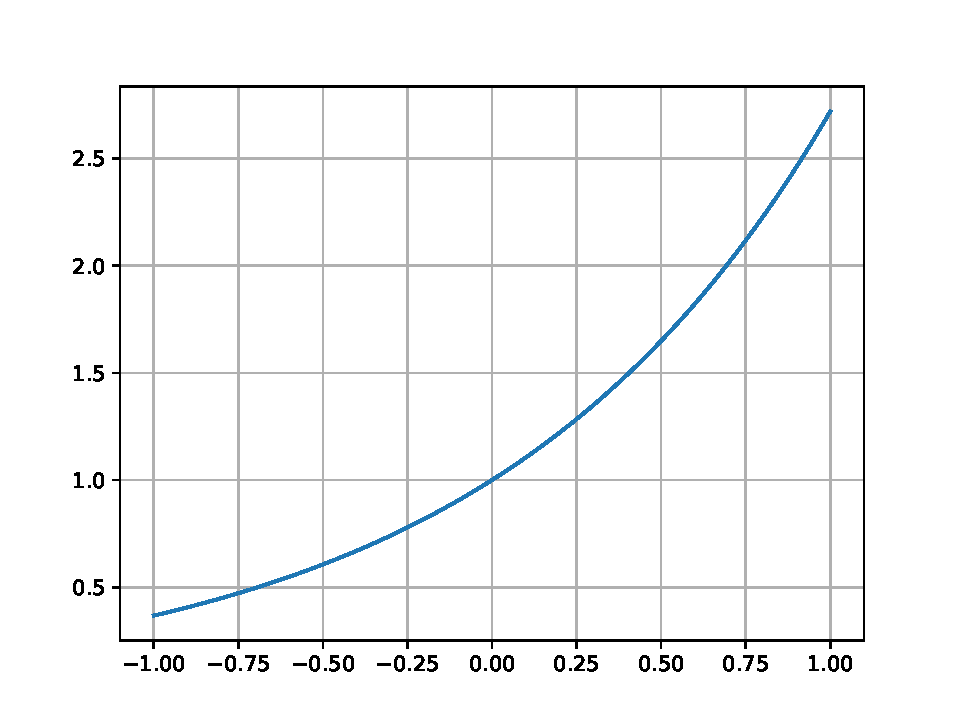
\includegraphics[width=\textwidth]{pic.pdf}
\end{figure}

Please ensure that the file \texttt{pic.pdf} is located within the \texttt{docs/tex/gfx} directory, as indicated by the path: \verb|docs/tex/gfx/pic.pdf|

\section*{Referencing to figures}
To reference to a specific figure, such as \ref{fig:my-fig}, you can use 
\begin{verbatim}
\ref{fig:my-fig}
\end{verbatim}


\section*{Citing}
To reference a particular source within your document, use the command 
\begin{verbatim}
\cite{Aastroem2000Modeluncertain}
\end{verbatim}
which will appear as \cite{Aastroem2000Modeluncertain}.

Remember to include the command \verb|\printbibliography| at the conclusion of your document; this is crucial for compiling the bibliography section.

\printbibliography

\end{document}